\documentclass[a4paper, 10pt, twoside]{article}
\usepackage[left=3cm, right=3cm, top=3cm, bottom=3cm]{geometry}
\usepackage[super]{natbib}
\usepackage{amsmath}
\usepackage[shortlabels]{enumitem}
\usepackage{bbold}
\usepackage{graphicx}
\usepackage{url}
\usepackage{hyperref}
\hypersetup{
    colorlinks=true,
    linkcolor=blue,
    filecolor=magenta,      
    urlcolor=cyan,
}


\begin{document}

\title{High Performance Computing - Micro Aevol}
\author{T\'eo Bouvard}
\maketitle

\section{Introduction}

Micro Aevol est une version réduite du modèle biologique Aevol \cite{aevol}, dont l'objectif est d'étudier le processus d'évolution à l'aide de la simulation d'organismes. Cette modèle réduit a pour but d'étudier l'optimisation de la performance du code sous-jacent au modèle.

\section{Version CPU}

Dans cette partie, on étudie l'optimisation la version CPU du code d'Aevol.
Pour le benchmark de \textit{strong scaling}, le processeur utilisé est un AMD Ryzen 7 3700X avec 32GB de RAM, le code est compilé à l'aide de CMake 3.19.1, g++ 10.2.0 et OpenMP 4.5 (201511)
Pour le benchmark de \textit{weak scaling}, le processeur utilisé est un Intel Core i7-9700 avec 16GB de RAM, le code est compilé à l'aide de CMake 3.13.14, g++ 8.3.0 et OpenMP.

\subsection{Analyse}

Afin de se familiariser avec le code, il est intéressant de profiler son exécution. Cela permet d'identifier la structure globale du programme ainsi que son chemin critique.

\begin{figure}[htpb]
	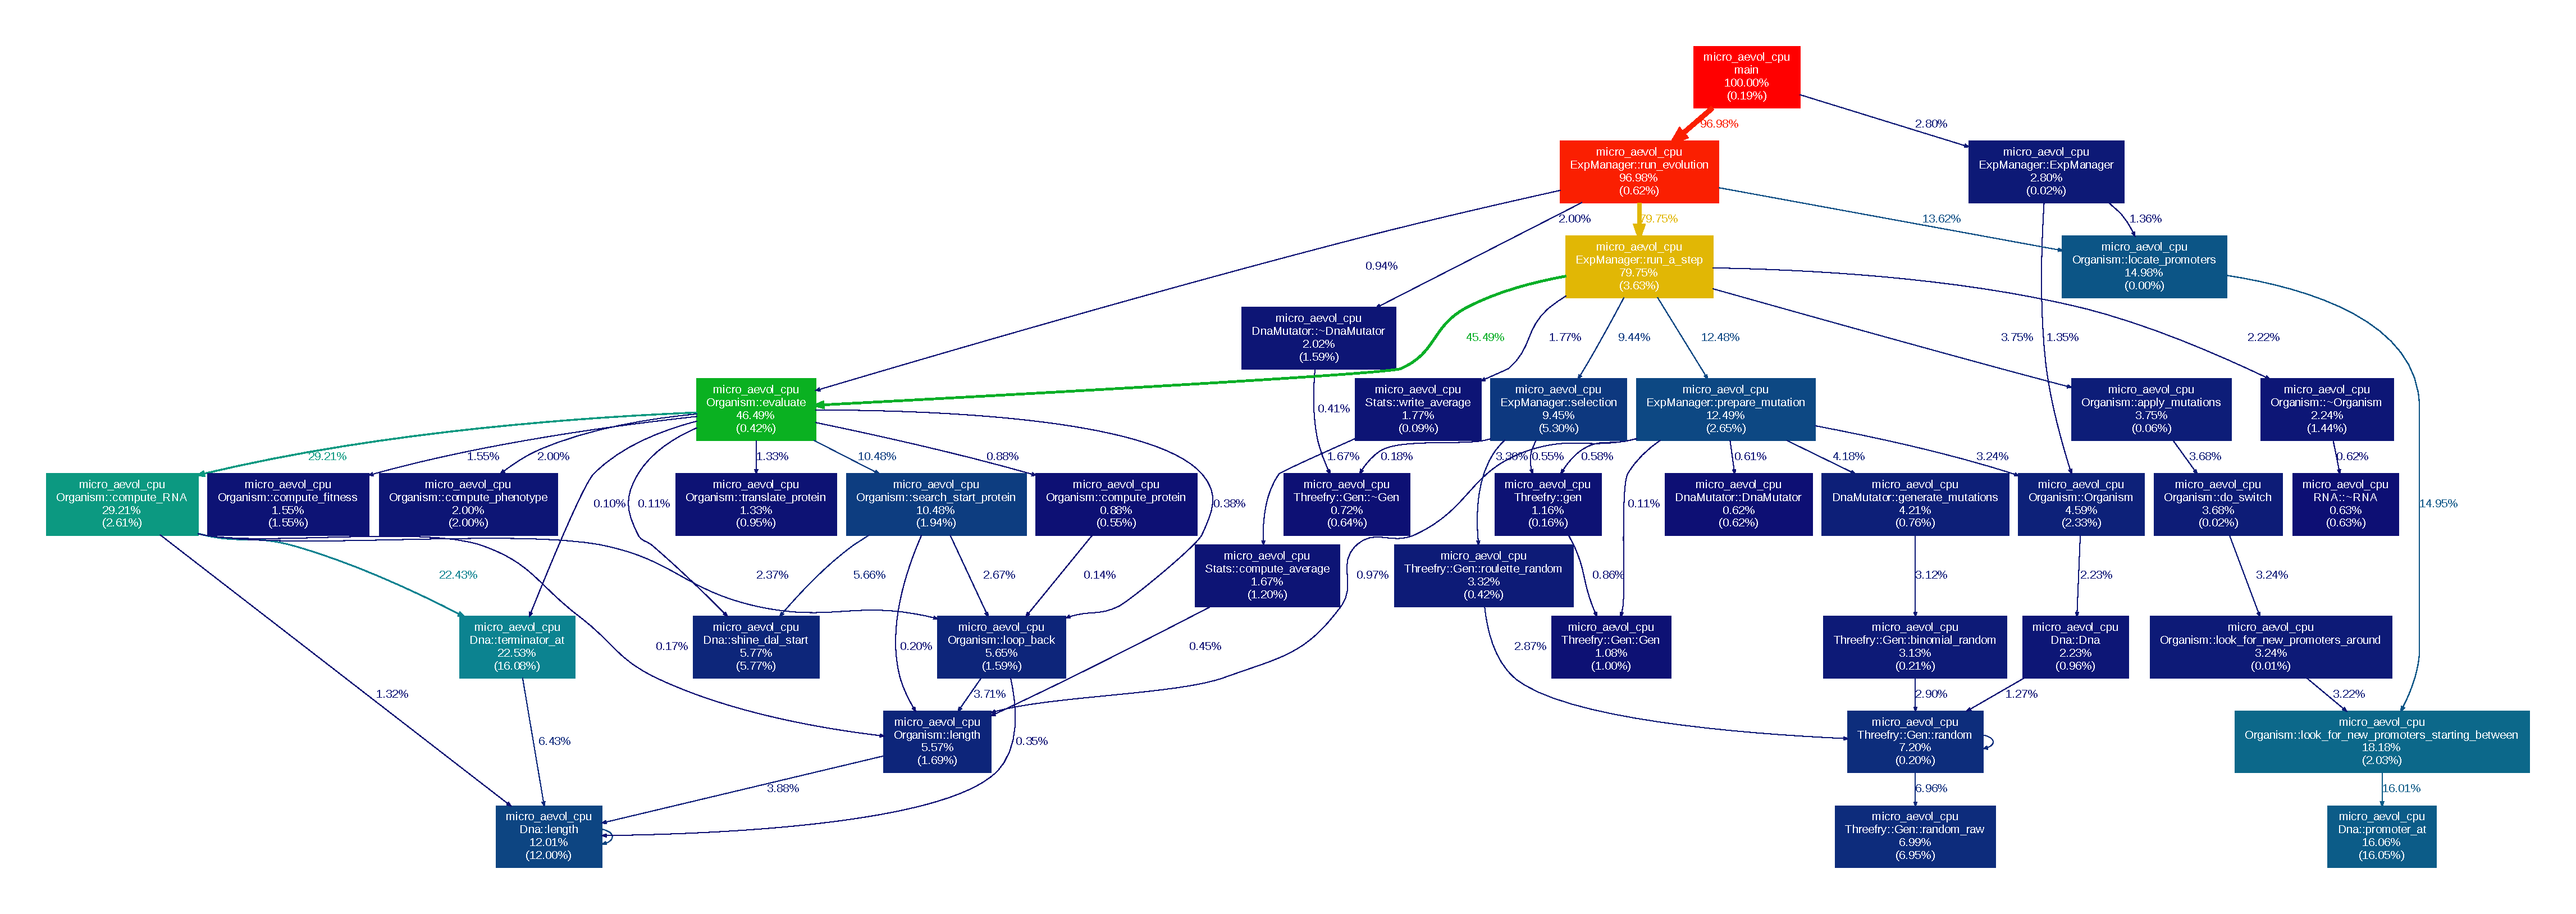
\includegraphics[width=\linewidth]{img/profile_aevol.pdf}
	\caption{Profilage de l'application avec les paramètres par défaut à l'aide de \textit{perf}}
\end{figure}

Dans le cas d'Aevol, on remarque que la fonction \textit{run\_a\_step} est exécutée pour chaque pas de temps de \textit{run\_evolution}, dont le nombre d'itérations est spécifié par l'argument \textit{n\_steps}.
Dans cette fonction, les différentes étapes du modèle biologique sont exécutées pour chaque organisme.

\subsubsection*{Parallélisation du modèle}

Toutes les étapes de ce modèle sont indépendantes pour chaque organisme sauf l'étape de sélection qui requiert la lecture de l'état des organismes voisins sur la grille. Une optimisation naturelle est donc de paralléliser le traitement de chaque organisme\label{parallel/orga}.

\subsubsection*{Échange de population}

Pour effectuer la phase d'échange des populations lors du passage d'un pas de temps au suivant, il peut être plus performant d'échanger les pointeurs sur les grilles d'organismes plutôt que de copier chaque organisme dans une boucle.

\subsubsection*{Latence du disque}

Une autre simple optimisation est de limiter les appels à \textit{printf}, qui ralentissent l'exécution de manière significative lorsque ces derniers sont très fréquents. En effet, en utilisant les arguments par défaut on diminue de moitié le temps d'exécution en redirigeant la sortie standard ainsi que la sortie d'erreur vers \textit{/dev/null}. Bien évidemment, cette optimisation n'est pas aussi significative lorsque l'on utilise des tailles de problèmes plus élevées, mais il est sage d'éviter des appels systèmes coûteux lorsqu'ils ne sont pas nécessaires. Une alternative à la redirection des streams serait d'ajouter un argument permettant de contrôler la verbosité du programme, et ainsi s'affranchir du coût de tous ces appels systèmes lors d'une exécution en mode silencieux.

De manière similaire, les écritures dans les fichiers de statistiques invoquant \textit{std::endl} ou \textit{std::flush} imposent la synchronisation des flux de sortie, ce qui peut avoir un coût d'appel système assez élevé lié à la lenteur de l'écriture sur disque. Une meilleure solution serait de stocker les statistiques en mémoire jusqu'au point de backup afin de les écrire dans des fichiers d'un seul coup, ce qui améliorerait le buffering déjà proposé par l'OS.

\subsection{Implémentation}

Dans l'optique de mesurer uniquement l'optimisation de la performance du modèle biologique, les benchmarks qui suivent n'incluent pas le temps d'écriture des fichiers de backup. En effet, cette écriture est réalisée par un seul thread et peut nécessiter la compression DEFLATE de plusieurs GB de données à l'aide de zlib, ce qui influe de manière significative sur le temps d'exécution du programme. Cependant, c'est un coût qui n'est pas directement lié au modèle biologique que l'on cherche à optimiser, et qui n'est effectué qu'à chaque point de backup. Si l'on souhaitait optimiser cette partie du programme, il serait utile d'utiliser un algorithme de compression plus performant que DEFLATE tel que \textit{lz4} ou \textit{zstd}. Comme on peut l'observer sur la figure \ref{fig:compression/tools}, l'utilisation de zstd 1.4.3 peut multiplier par 4 la vitesse de compression maximale de zlib tout en améliorant le ratio de compression de 36.4\% à 34.7\%. Si l'on se permet de sacrifier de la mémoire pour gagner en performance, on peut multiplier par 7 (respectivement 10) la vitesse de compression en obtenant un ratio de compression de 50.5\% (respectivement 62.1\%).

\begin{figure}[htb]
	\centering
	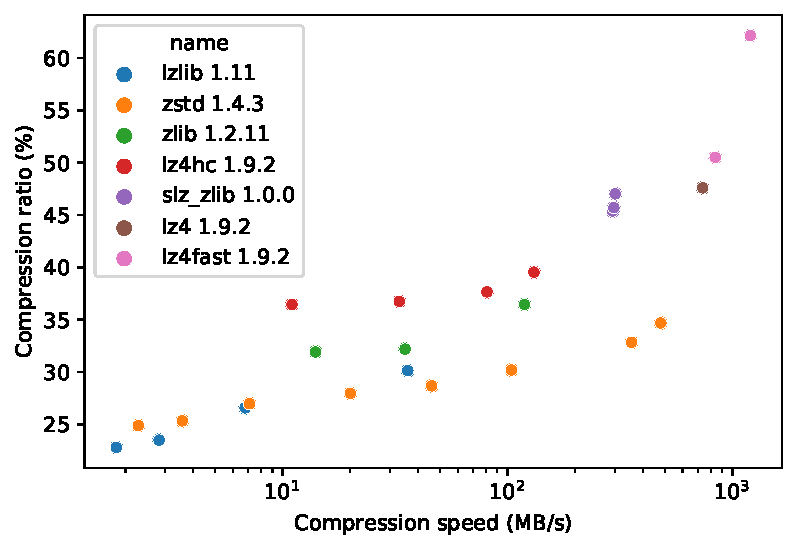
\includegraphics[width=0.5\linewidth]{img/compression_tools.pdf}
	\caption{Comparaison d'outils de compression sur le corpus Silesia \cite{lzbench}}
	\label{fig:compression/tools}
\end{figure}

De manière similaire, le passage à l'échelle n'est mesuré que pour des tailles de problèmes tenant en mémoire. Au delà d'une taille de population supérieure à $512 \times 512$ et d'un génome de taille supérieure à 50000 gènes, la taille des structures de données dépasse la capacité des 32 GB de RAM, et la mesure des temps d'exécution serait influencée par la vitesse du disque utilisé en swap.

\subsubsection{Parallélisation du modèle}

Chaque boucle itérant sur l'ensemble des organismes de la simulation est parallélisée à l'aide d'une directive \textit{omp parallel for}, en utilisant un scheduling statique. Ce choix de scheduling provient de l'observation de la répartition des charges de calcul sur les différents organismes.

\begin{itemize}
	\item Lors des phases de sélection, de swap de population et de recherche de meilleur individu, les calculs sont identiques pour chaque organisme.
	\item La phase d'évaluation n'est effectuée que si l'organisme a subi une mutation, ce qui est lié à un processus aléatoire. De plus, cette phase est d'autant plus coûteuse que le nombre de mutations subies est élevé. Cependant, chaque organisme est soumis au même processus aléatoire de mutation, ce qui répartit les mutations de manière uniforme dans la population.
\end{itemize}

Ces deux observations suggèrent que la charge de calcul est répartie de manière uniforme sur l'ensemble de la population, et qu'il sera donc plus performant de diviser le traitement en chunks de taille égale plutôt que d'opter pour des stratégies de scheduling dynamiques ou guidées qui nécessiteraient un overhead inutile dans ce cas particulier.

\begin{figure}[htb]
	\centering
	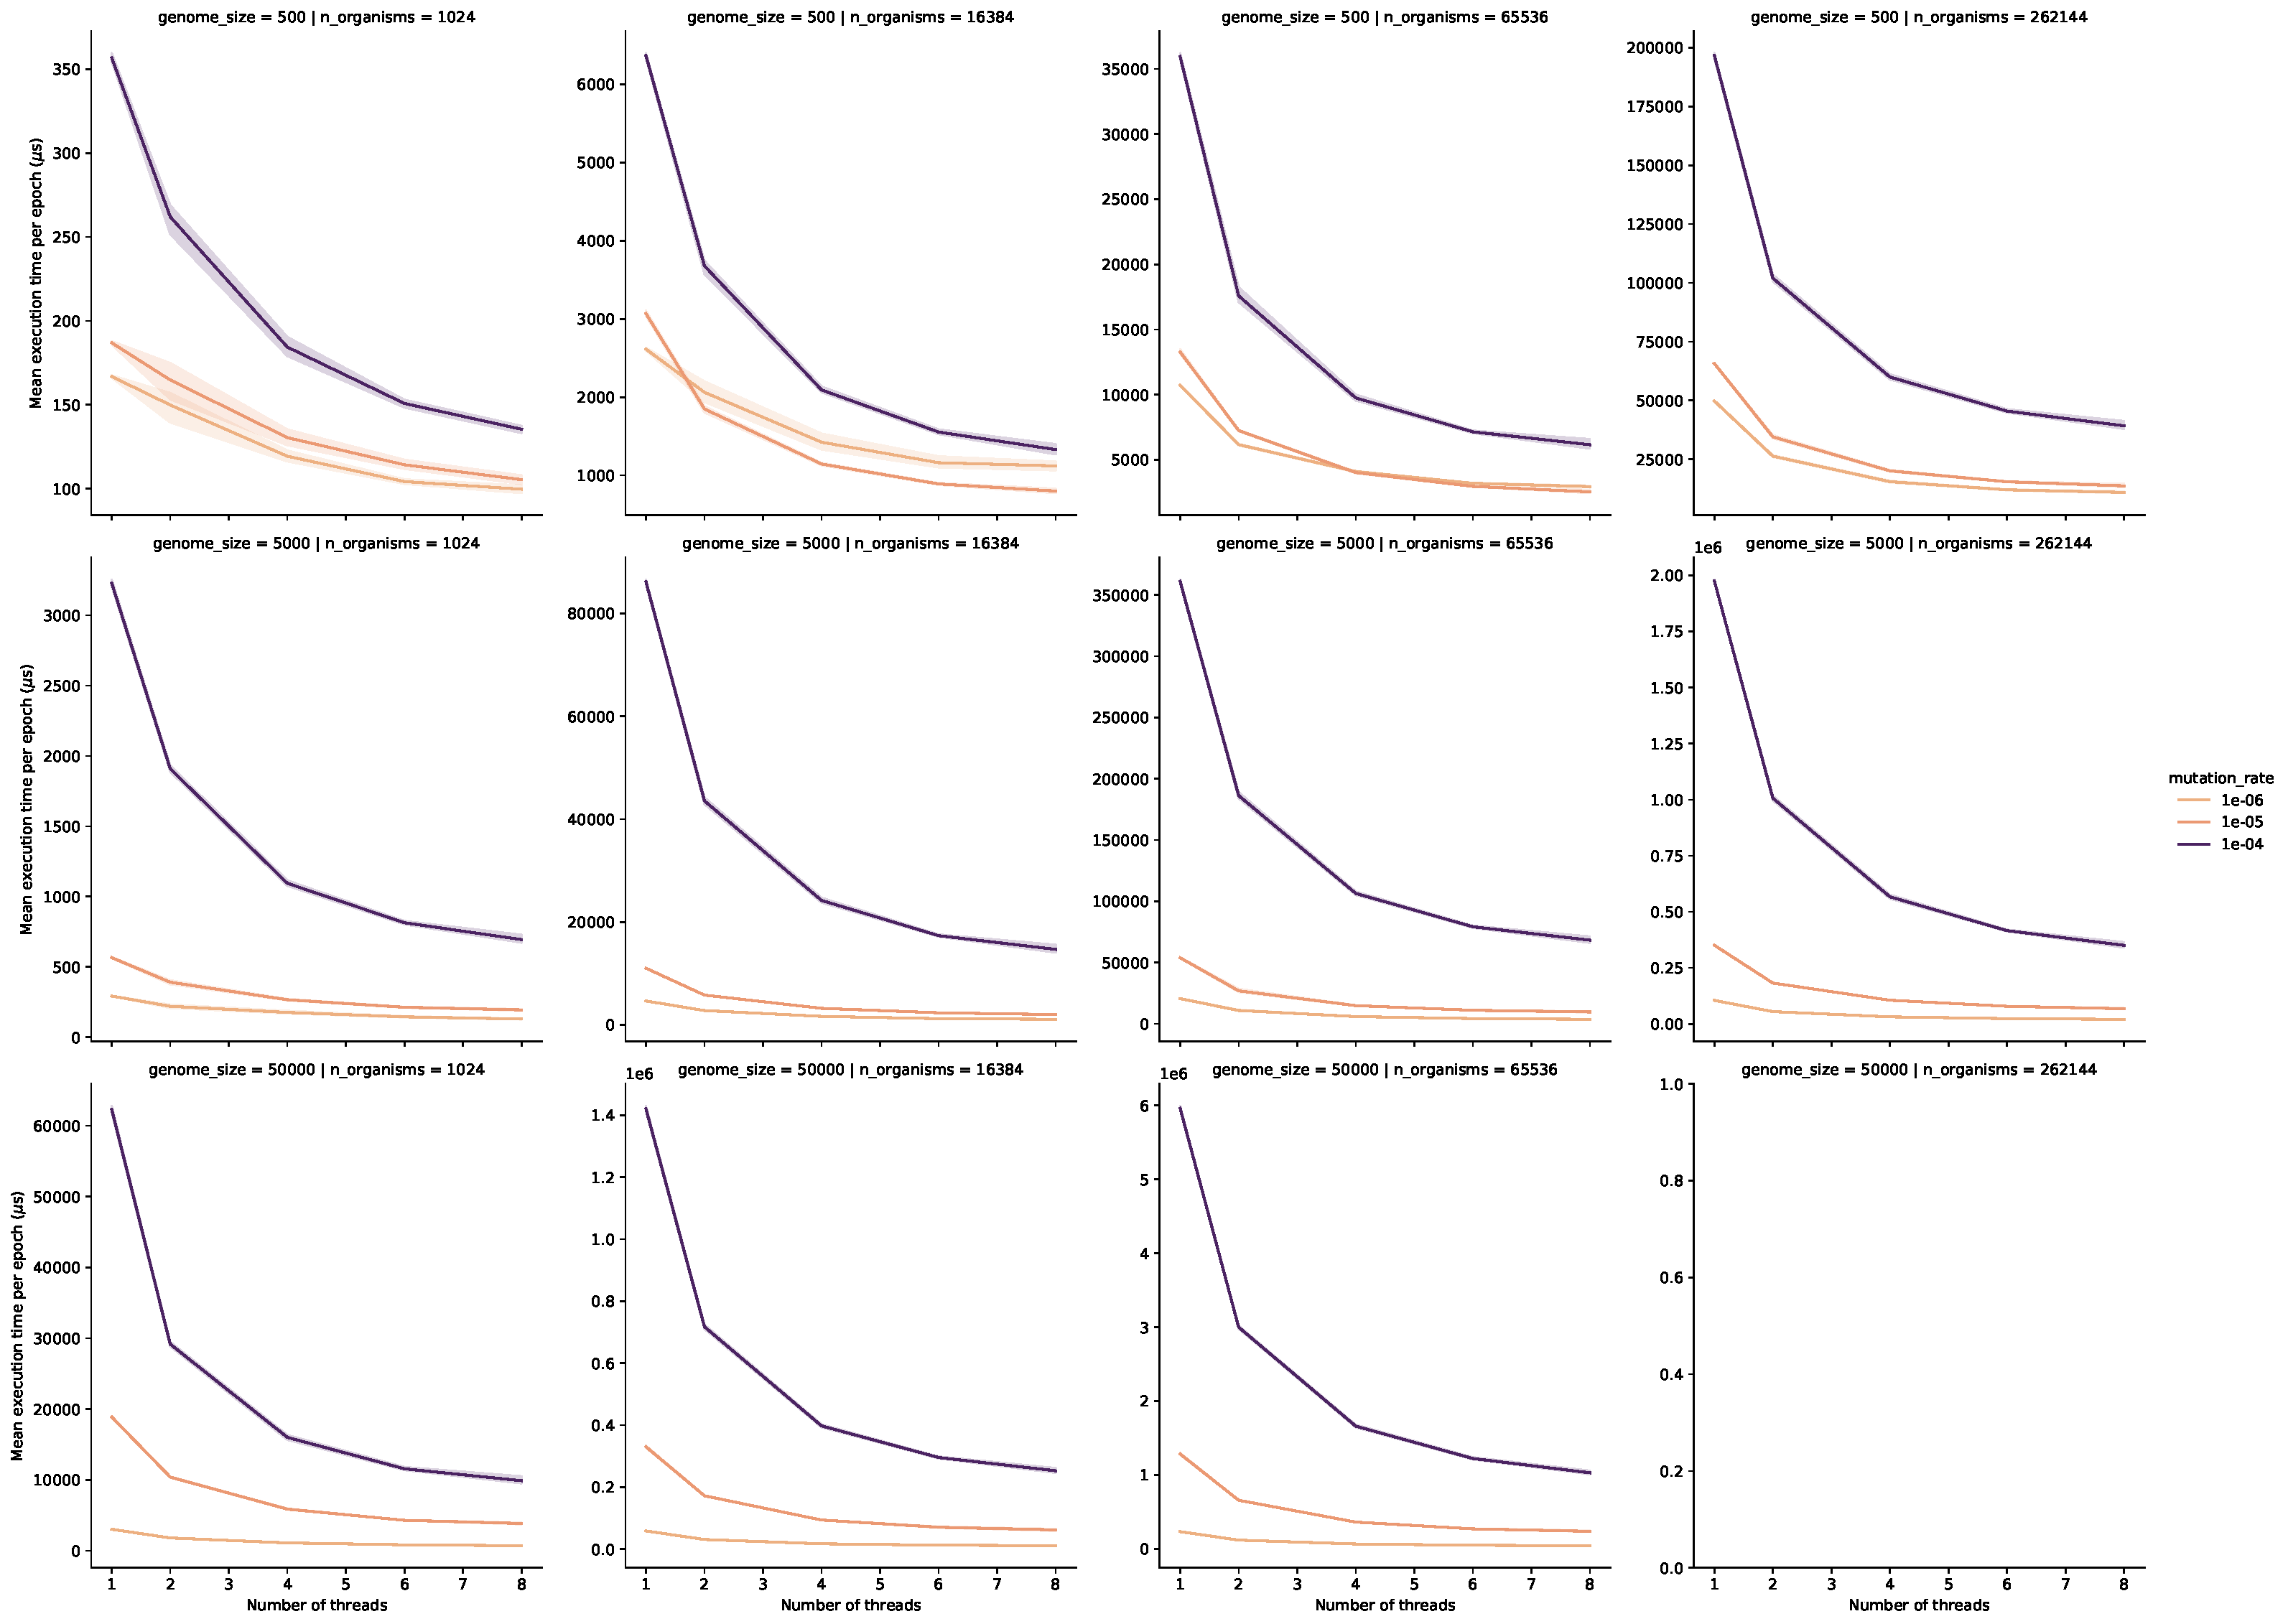
\includegraphics[width=0.7\linewidth]{img/benchmark_omp_static.pdf}
	\caption{Benchmarks de la parallélisation du modèle biologique à l'aide d'OpenMP}
	\label{fig:benchmarks/omp}
\end{figure}

Sur la figure \ref{fig:benchmarks/omp}, la première observation qui peut être réalisée est que toutes choses étant égales par ailleurs, le temps d'exécution du programme augmente avec le taux de mutation. Cela s'explique par la phase d'évaluation qui n'est effectuée qu'en cas de mutation. On observe que cette stratégie de paraléllisation fonctionne, car le temps d'exécution est inversement proportionnel au nombre de threads utilisés.

\subsubsection*{Strong scaling}

Le speedup de cette parallélisation est mis en évidence sur la figure \ref{fig:speedup/omp}, qui visualise le gain de temps sur différentes tailles de problèmes pour un nombre croissant de threads.
Ce speedup $S$ est défini par $ S_n = \frac{t_1}{t_n} $, où $n$ représente le nombre de threads et $t$ le temps d'exécution.

\begin{figure}[htb]
	\centering
	\begin{minipage}{0.32\textwidth}
		\centering
		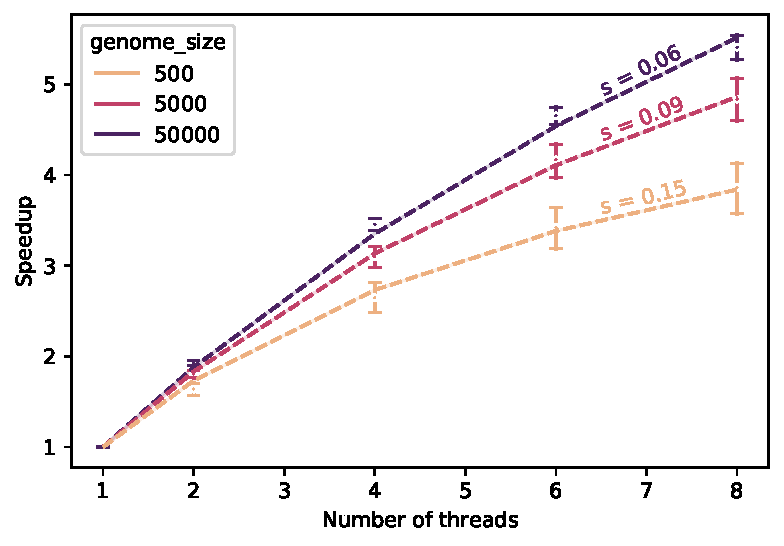
\includegraphics[width=\textwidth]{img/speedup_genome_size.pdf}
	\end{minipage}
	\begin{minipage}{0.32\textwidth}
		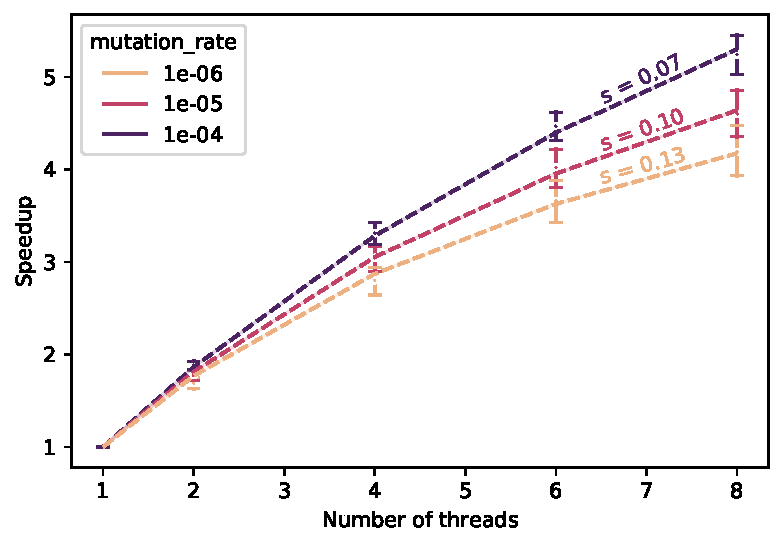
\includegraphics[width=\textwidth]{img/speedup_mutation_rate.pdf}
	\end{minipage}
	\begin{minipage}{0.32\textwidth}
		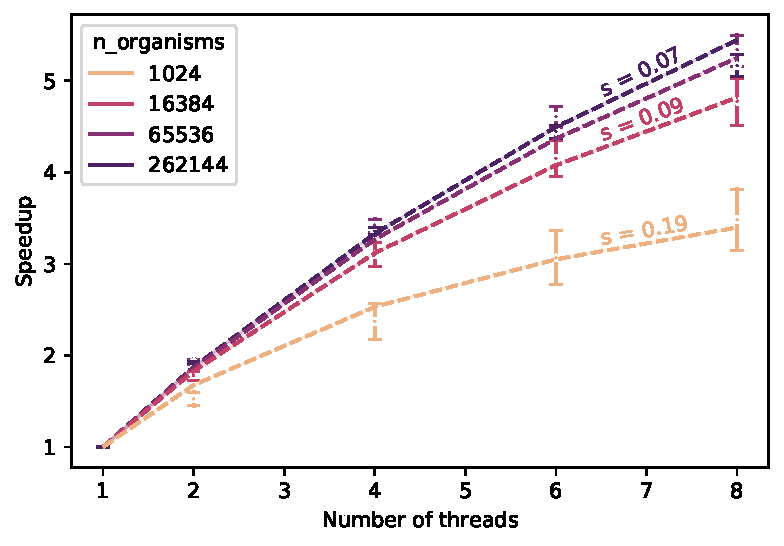
\includegraphics[width=\textwidth]{img/speedup_n_organisms.pdf}
	\end{minipage}
	\caption{Speedup de la parallélisation du modèle biologique à l'aide d'OpenMP}
	\label{fig:speedup/omp}
\end{figure}

On remarque une accélération d'un facteur de 5 pour une multiplication par 8 du nombre de threads. Cette accélération n'est pas linéairement proportionnelle au nombre de threads car le code contient des parties intrinsèquement séquentielles qui ne peuvent être parallélisées. On observe plutôt un speedup de la forme

$$ S = \frac{1}{s + \frac{1-s}{n}} $$

où $s$ représente le temps nécessaire à l'exécution de la partie séquentielle du code, $1-s$ le temps nécessaire à l'exécution de la partie parallèle et $n$ le nombre de threads utilisés.

Ce phénomène a été théorisé par Amdahl \cite{amdahl2007validity} et est connu aujourd'hui sous le nom de loi d'Amdahl.
Pour chaque valeur des différentes variables, on détermine $s$ à l'aide d'une régression par moindres carrés de la loi d'Amdahl sur les données obtenues lors des benchmarks.

Ces valeurs de $s$ nous permettent de déterminer le speedup théorique maximal pour les tailles de problèmes étudiées. Par exemple, pour un génome comportant 50000 gènes, on peut calculer

$$ S_{max} = \lim_{n\to\infty} \frac{1}{0.06 + \frac{0.94}{n}} = 16.7 $$

cependant, si l'on fixe la taille du génome à 5000 gènes, on obtient un speedup théorique maximal de

$$ S_{max} = \lim_{n\to\infty} \frac{1}{0.15 + \frac{0.85}{n}} = 6.7 $$

On en conclue que pour obtenir un speedup maximal en utilisant cette parallélisation, il est nécessaire d'utiliser des tailles de génome et de population les plus grandes possibles. Cependant, on en conclue aussi que plus le taux de mutation est élevé, moins la parallélisation est efficace, ce qui indiquerait la nécessité d'étudier une autre stratégie de parallélisation pour la méthode \textit{evaluate} pour des taux de mutation élevés.

\subsubsection*{Weak scaling}

Le paradigme d'analyse du speedup utilisant des tailles de problème fixées, proposé par Amdahl, n'est cependant pas le seul moyen de quantifier l'efficacité de la parallélisation. L'observation théorisée par Gustafson \cite{gustafson} est que l'utilisation d'un plus grand nombre de processeurs permet de résoudre des problèmes de taille plus grande. Selon lui, une métrique plus pertinente est le scaled speedup $S'$, défini de la manière suivante

$$ S' = s + (1 - s) \times n$$

\begin{figure}[htb]
	\centering
	\begin{minipage}{0.45\textwidth}
		\centering
		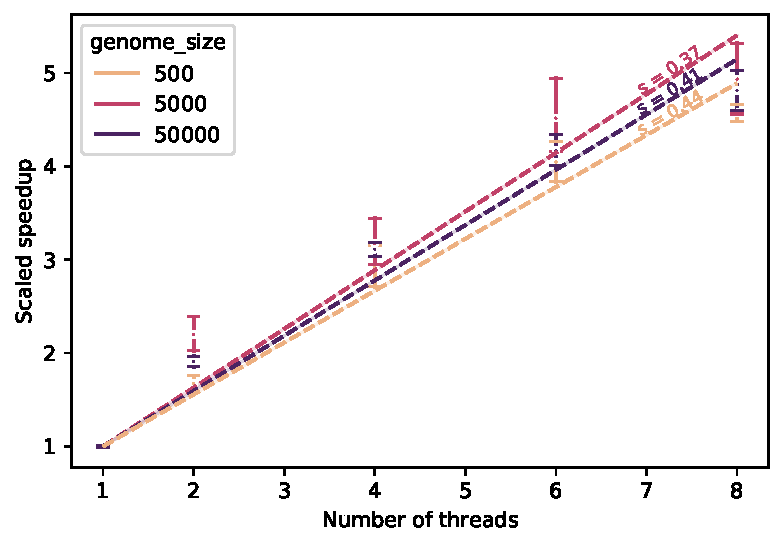
\includegraphics[width=\textwidth]{img/weak_speedup_genome_size.pdf}
	\end{minipage}
	\begin{minipage}{0.45\textwidth}
		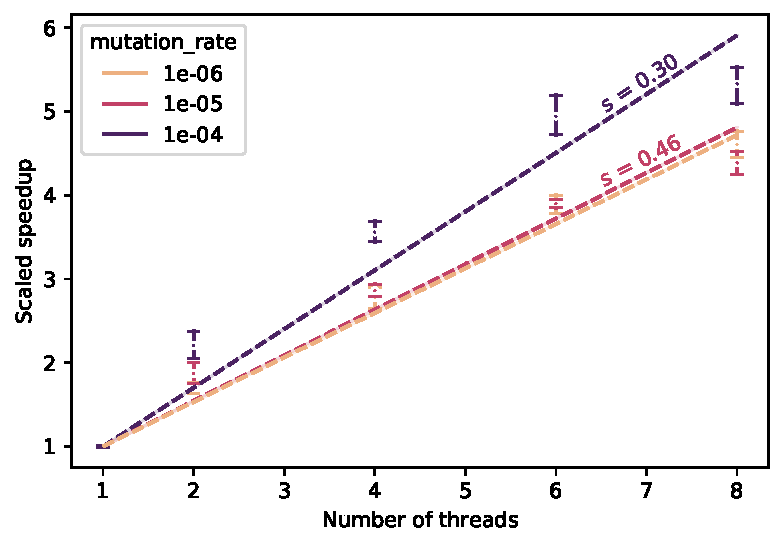
\includegraphics[width=\textwidth]{img/weak_speedup_mutation_rate.pdf}
	\end{minipage}
	\caption{Scaled speedup de la parallélisation du modèle biologique à l'aide d'OpenMP}
	\label{fig:scaled-speedup/omp}
\end{figure}

Le scaled speedup quantifie le temps qu'il faudrait à un seul thread pour exécuter le programme que l'on exécute à l'aide de plusieurs threads. La figure \ref{fig:scaled-speedup/omp} montre l'évolution de ce scaled speedup lorsque l'on fixe différentes variables. Sur cette figure, on observe la tendance linéaire de la loi de Gustafson jusqu'à 6 threads, mais on remarque un effondrement du speedup lors de l'utilisation de 8 threads.

Contrairement à la loi d'Amdahl qui restreint le speedup maximal atteignable pour une taille de problème fixée, la loi de Gustafson nous fournit une métrique plus encourageante qui ne limite pas le speedup théorique, car l'ajout de nouveaux threads nous permettra de résoudre des problèmes toujours plus grands.

% Cette perte d'efficacité à 8 threads peut être liée à une saturation du CPU utilisé, qui possède 8 coeurs logiques. Pour rappel, les résultats de ce benchmark ne sont pas comparables à ceux effectués pour le strong scaling car ils n'ont pas été effectués sur la même machine. La machine utilisé pour réaliser ce benchmark est partagée par plusieurs utilisateurs (tandis que l'autre ne l'était pas) et l'OS a peut-être limité le temps de scheduling disponible pour ce benchmark pour permettre à d'autres programmes d'utiliser du temps CPU.

La figure \ref{fig:speedup-models} offre une comparaison de l'approche d'Amdahl et de Gustafson pour quantifier le speedup d'un programme parallélisé.

\begin{figure}[htb]
	\centering
	\begin{minipage}{0.33\textwidth}
		\centering
		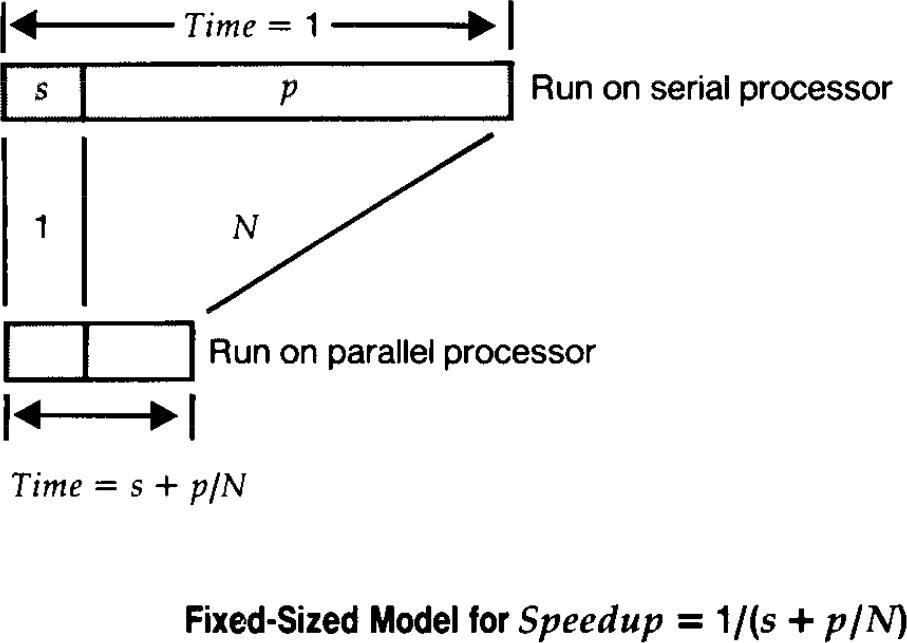
\includegraphics[width=\textwidth]{img/amdahl_speedup_model.png}
	\end{minipage}
	\begin{minipage}{0.65\textwidth}
		\centering
		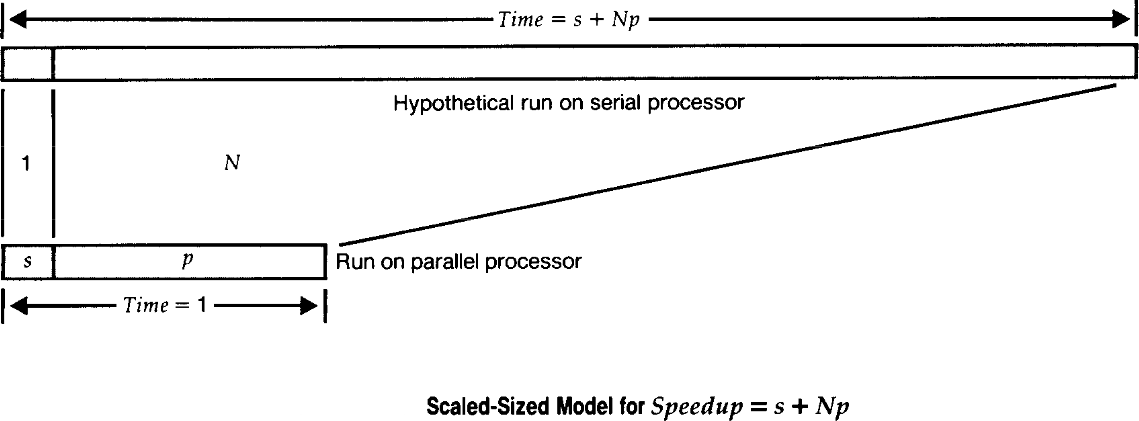
\includegraphics[width=\textwidth]{img/gustafson_speedup_model.png}
	\end{minipage}
	\caption{Modèles à taille de problème fixe (Amdahl) et à temps d'exécution fixe (Gustafson)}
	\label{fig:speedup-models}
\end{figure}

\subsubsection{Échange de population}

La figure \ref{fig:swap/strat} montre la distribution du temps par époque pour deux stratégies d'échange de population.
La première stratégie \textit{for\_swap} consiste à itérer sur les organismes de la population et d'échanger les génomes de la génération $n$ et $n-1$.
La seconde stratégie \textit{pointer\_swap} consiste à échanger directement les pointeurs sur les populations de la génération $n$ et $n-1$.
On suppose que la taille du génome ainsi que celle de la population peuvent avoir une influence sur la performance de cette optimisation, ainsi la figure \ref{fig:swap/strat} présente les temps d'exécution pour le nombre total de gènes, défini par

$$ n_{genes} = n_{organismes} \times taille_{genome} $$

\begin{figure}[htb]
	\centering
	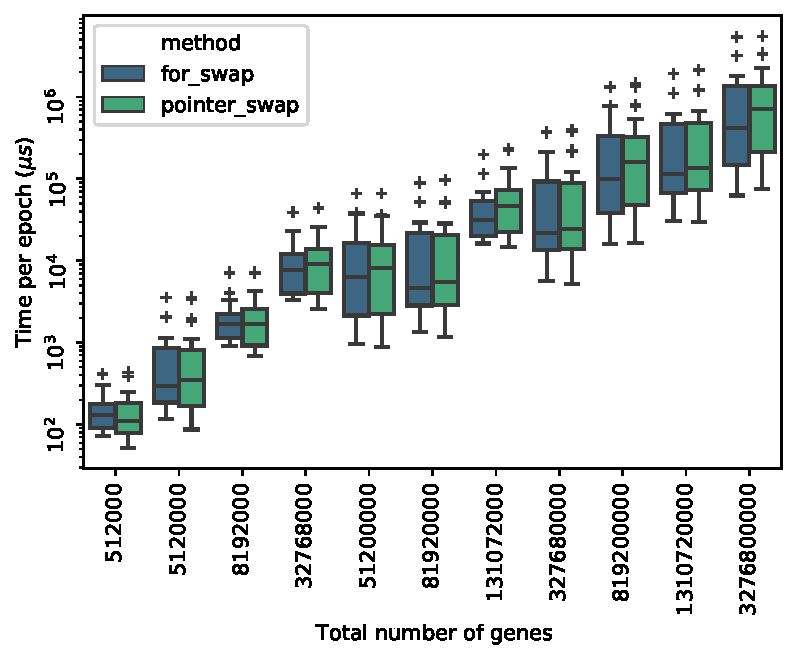
\includegraphics[width=0.5\linewidth]{img/swap_strategies.pdf}
	\caption{Stratégies d'échange de population}
	\label{fig:swap/strat}
\end{figure}

Bien que la meilleure performance par taille de problème soit généralement atteinte par l'échange de pointeurs, on observe que la performance médiane de cette stratégie est statistiquement moins bonne que celle de la boucle d'échange.
L'hypothèse émise est que le compilateur est capable de fournir une optimisation de la boucle d'échange au moins aussi bonne que la stratégie du \textit{pointer\_swap}.

\section{Version GPU}

Dans cette partie, on étudie l'optimisation la version GPU du code d'Aevol. Le processeur utilisé est un Intel Core i7-9700 avec 16GB de RAM, le code est compilé à l'aide de CMake 3.13.14, g++ 8.3.0 et nvcc 9.2.

\subsection{Analyse}

De même que pour la version CPU, on analyse le comportement du programme en profilant son exécution. Le profiler NVVP nous indique que le kernel \textit{evaluate\_population} occupe 99.7\% du temps d'exécution. On observe sur la figure \ref{fig:kernel/timings} la logarithme du temps d'exécution moyen de chaque kernel constituant le modèle.

\begin{figure}[htp]
	\centering
	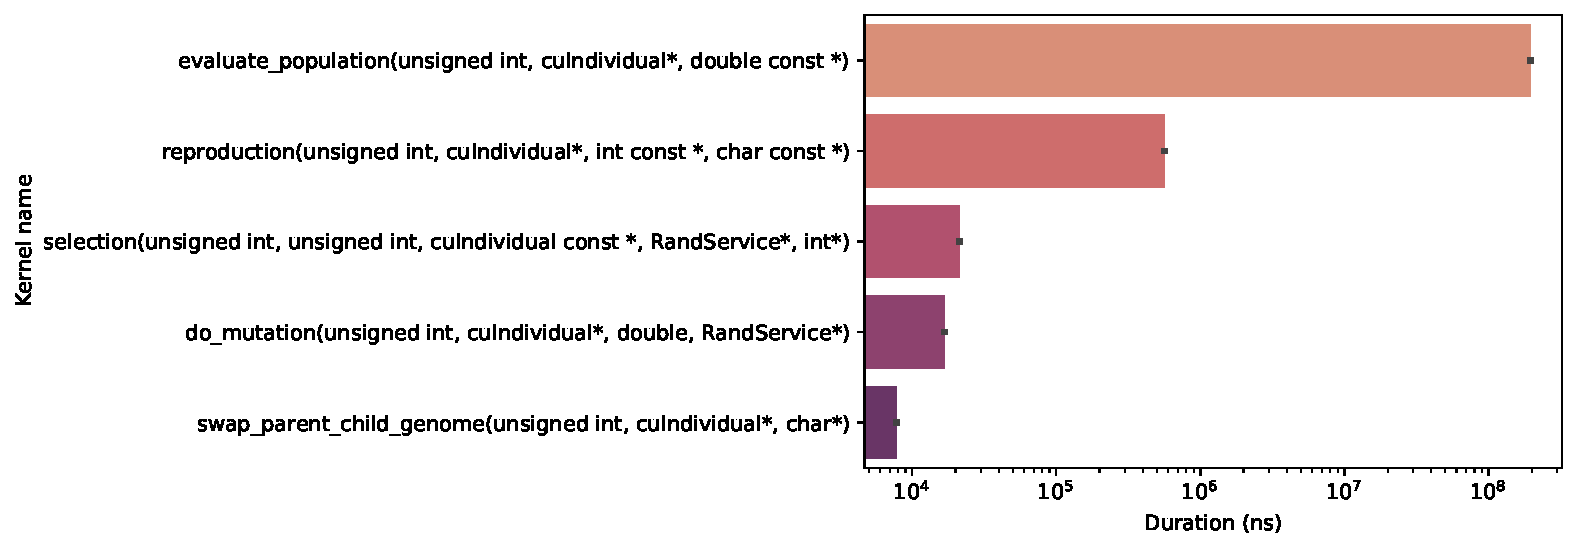
\includegraphics[width=0.7\linewidth]{img/kernel_timings.pdf}
	\caption{Logarithme du temps d'exécution moyen de chaque kernel}
	\label{fig:kernel/timings}
\end{figure}

Ce temps d'exécution important s'explique principalement par le haut degré de divergence dans le code de ce kernel. En effet, certaines parties du kernel sont systématiquement exécutées par un seul thread dans chaque warp, ce qui augmente significativement le nombre d'instructions devant être exécutées par chaque warp \cite{nvidia/branching}.

Afin de profiler davantage les kernels les plus couteux pour identifier plus précisément les phases de divergence inter-warp, il était nécessaire de bénéficier des privilèges administrateur, qui ne nous sont pas accordés sur les machines du département.

\bibliographystyle{unsrtnat}
\bibliography{report}

\end{document}
